%------------------------------------------------------------
% Description : Важные формулки, просто так
% Author      : Iliya Tikhonenko <iliya.t@mail.ru>
% Created at  : Sat Jun 17 14:33:58 MSK 2017
%------------------------------------------------------------
\documentclass[draft,landscape,timbord]{notes}
\usepackage{tmath}
\usepackage{cussymb}
\usepackage{multicol}
\geometry{
  left=1cm,
  right=1cm,
  top=1cm,
  bottom=1cm
}
\graphicspath{{img/}}
\everymath{\displaystyle}
\setlist[itemize,1]{leftmargin=0cm, noitemsep, label=$\triangleright$}

\begin{document}
\begin{multicols*}{3}
\begin{enumerate}
  \item 
    \begin{description}
      \item[$\v r$:] $\v r(t)$, $(x,y,z)(t)$, $\v r(s)$.
      \item[$\dot{\v r}$:] $\dot{\v r}(t)$, $(\dot x,\dot y,\dot z)(t)$, $\v\tau \dot s$.
      \item[$\ddot{\v r}$:] $\ddot{\v r}(t)$, $(\ddot x,\ddot y,\ddot z)(t)$,
        $\ddot s \v \tau + \dot s^2 k_1 \v n$
    \end{description}
  \item \quest
  \item В криволинейных координатах
    \begin{itemize}[$\triangleright$]
      \item $\v v = \sum_k \dot q^k \v {e_k}$
      \item $\v w = \sum_k \ddot q^k \v {e_k} + \sum_{k,i} \dot q^k \dot q^i \, \pder{\v{e_k}}{q^i}$
      \item ${w^j} = \ddot q^j + \sum_{k,i} \dot q^k \dot q^i \, \Gamma_{ki}^j$
      \item $ \Gamma_{j,\,ki} = \pder{\v{e_k}}{q^i}\cdot \v{e_j}$~--- I рода
      \item $ \Gamma_{ki}^j \;\,\,= \pder{\v{e_k}}{q^i}\cdot \v{e^j}$~--- II рода
      \item $w_\ell = 
        \fder{}{t} \left(\pder{}{\dot q^\ell}\left(\frac{\dot{\v r}^2}{2}\right)\right) 
        - \fder{}{q^\ell} \left(\frac{\dot{\v r}^2}{2}\right)$
    \end{itemize}
  \item Про углы Эйлера \\
    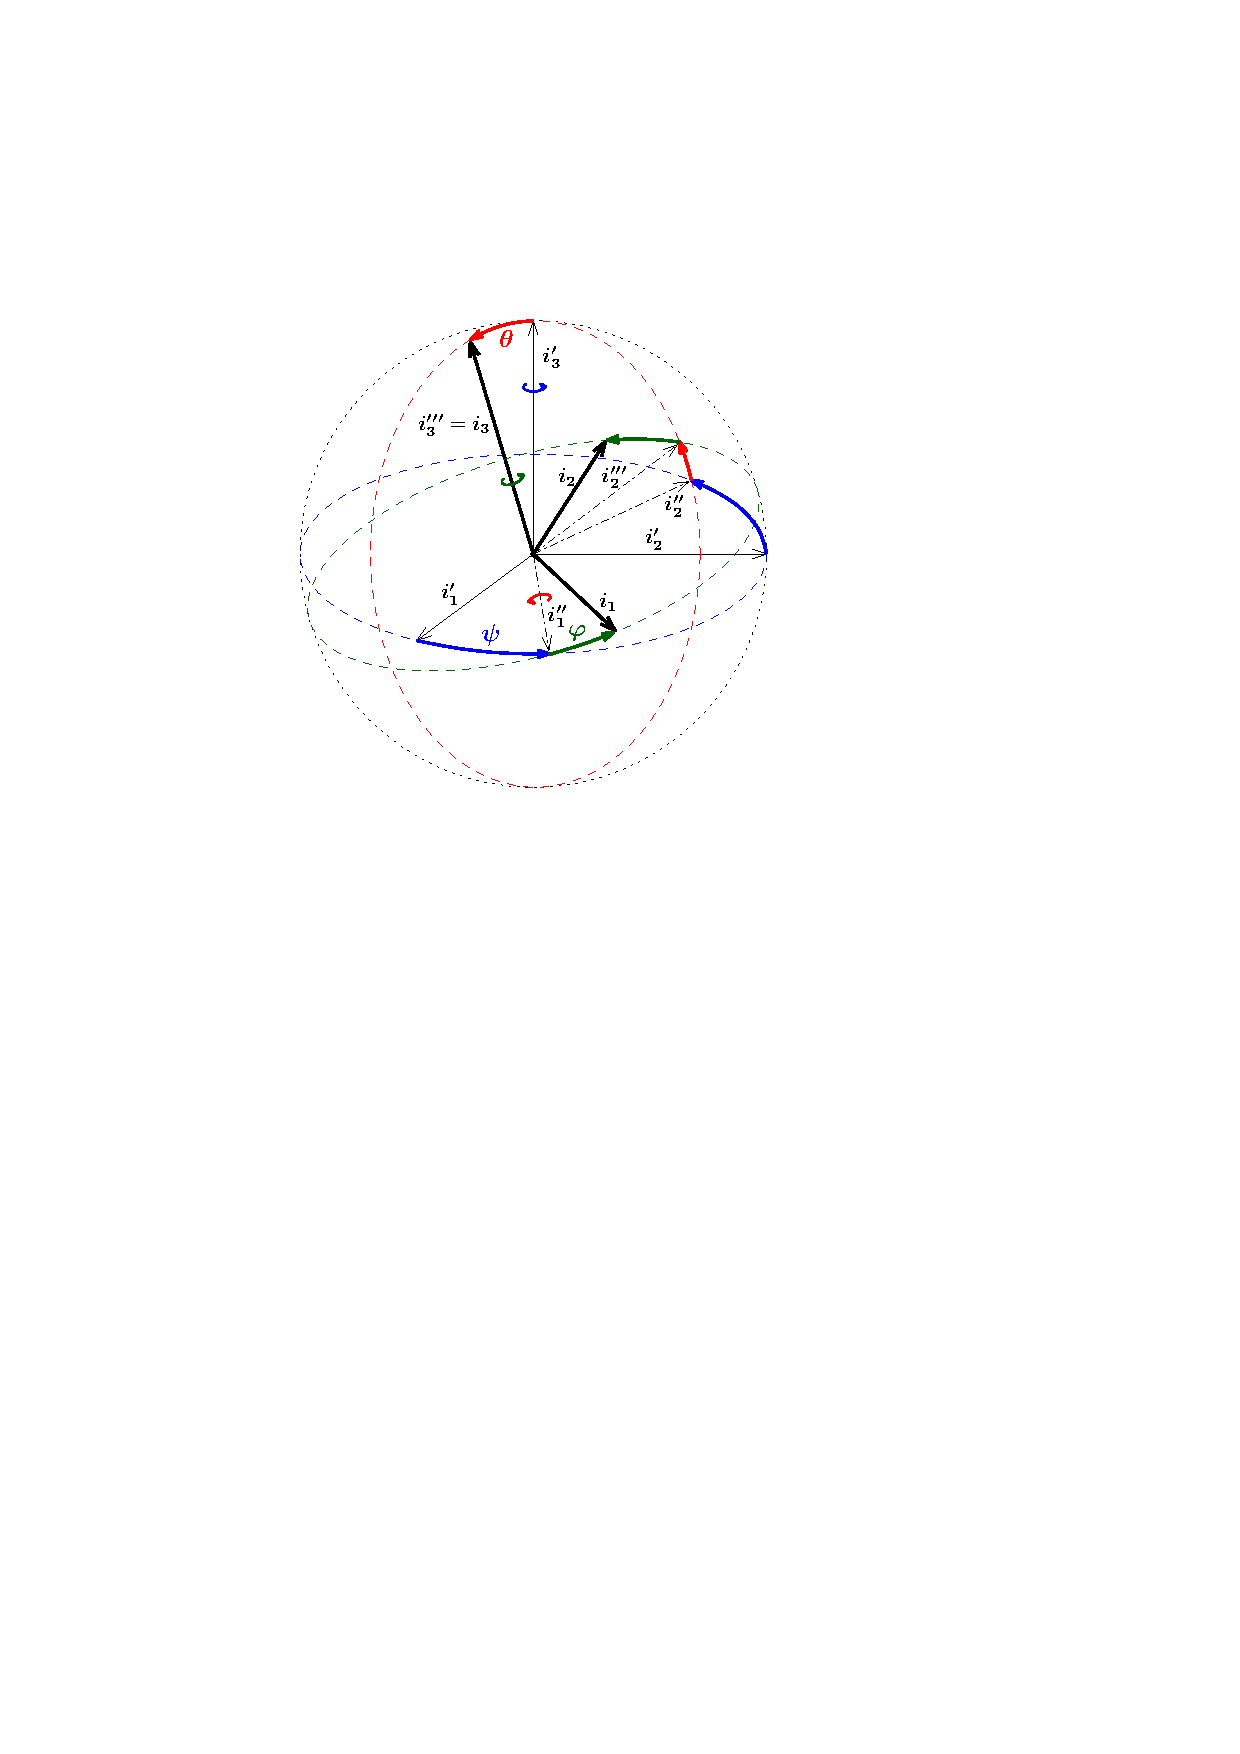
\includegraphics[width=1.0\linewidth]{euler_ang.pdf}

    \begin{itemize}[$\triangleright$]
      \item $\v \omega = \dot\psi\,\v{i_3'} + \dot\theta\,\v{i_1''} + \dot\varphi\,\v{i_3} $
      \item $\v R (t) = \v{R_0} (t) + \v r(t)$
      \item $\v v = \v {v_0} + \v{\omega \times r} + \v{v_r}$
      \item $\v w = \v w_0 + \dot{\v \omega} \times \v r 
        + \v \omega \times (\v \omega \times \v r) + 2 \v \omega \times \v{v_r} + \v{w_r}$
    \end{itemize}
  \item  
  \item  
  \item  
  \item  
  \item В поле центральной силы $\neg$
    \begin{itemize}[$\triangleright$]
      \item $u = 1/\rho$.
      \item  Формулы Бине \\
        $\left\{\begin{aligned}
          v^2 &= c^2 \left(\left(\fder{u}{\varphi}\right)^2 + u^2 \right) \\
          w_\rho &= -c^2 u^2 \left(\fder[2]{u}{\varphi} + u \right)
      \end{aligned}\right.$
    \item Невыразимая жжесть
    \end{itemize}
  \item \quest\flame Движение твёрдого тела $\neg$
    \begin{itemize}
    \raggedright
      \item $\omega =0$~--- поступательное
      \item $\v {v_0}, \v {w_0} =0, \omega = \dot \varphi \v{i_3}$~--- вращение вокруг неподвижной оси
      \item $\v {v_0} \coori \v{\omega}$~--- винт
      \item \quest Как попало вокруг неподвижной точки \footnote{У нас тут вроде косяк, 
        а дальше снова как здесь \sour} $\neg$ 
        $\begin{aligned}
          \v \omega 
          &= \v{i_1} (\dot \psi \sin \theta \sin \varphi + \dot \theta  \cos \varphi ) + \\
          &+ \v{i_2} (\dot \psi \sin \theta \cos \varphi - \dot \theta \sin \varphi ) + \\
          &+ \v{i_3} (\dot \psi \cos \varphi + \dot \varphi )
      \end{aligned}$
    \end{itemize}
  \item Скорость и ускорение точек твердого тела
    \begin{itemize}
      \item $\v v = \v {v_0} + \v {\omega \times r}$
      \item $\v w = \v {w_0} + \dot{\v\omega} \times \v r + \v\omega \times (\v\omega \times \v r)$
    \end{itemize}
  \item Сложение движений ТТ
    \begin{itemize}
      \item $\v {v_{r_n}} 
        = \sum_{k=0}^{n-1} \left( \v{v_k} + \v{\omega_k} \times \ov{->}{O_kO}\right) 
        + \sum_{k=0}^{n-1} \v{\omega_k} \times \v{r_0}$
      \item $\v{V} = \sum_{k=0}^{n-1} \left( \v{v_k} + \v{\omega_k} \times \ov{->}{O_kO}\right) $
      \item $\Omega  = \sum_{k=0}^{n-1} \v{\omega_k} \quad\Rightarrow \v {v_{r_n}} 
        = \v V + \v\Omega \times \v{r_0}$
    \end{itemize}
  \item Кинематический винт
  \end{enumerate}
\end{multicols*}
\end{document}
% vim:tw=100 cc=100
